\documentclass[11pt,a4paper]{article}
\title{Next: Preliminary results from first floor CAD}
\usepackage{cite}
\usepackage{hyperref}
\usepackage{textcomp}
\usepackage{amssymb}
\usepackage{subcaption}
\usepackage{amsfonts}
\newcommand{\norm}[1]{\left\lVert#1\right\rVert}
\usepackage[left=2cm,right=2cm,top=2cm,bottom=3cm]{geometry}
\usepackage{amsmath}
\setlength\parindent{0pt}
\usepackage{float}
\usepackage{placeins}
\pretolerance=10000
\tolerance=2000
\emergencystretch=10pt
\author{Lucy Henley, Joshua Moore, Timothy Ostler \& Thomas Woolley\footnote{moorej16@cardiff.ac.uk, henleyl1@cardiff.ac.uk, ostlert@cardiff.ac.uk,woolleyt1@cardiff.ac.uk}}
\usepackage{graphicx}
\graphicspath{{./images_for_next/}}
\begin{document}
\maketitle

\section*{Key points}
\begin{itemize}
\item We have run our seat selection code over the old building first floor layout, based on the provided CAD file.
\item We achieved a maximum seat occupancy, with a $2$m social distancing measure, of approximately $45\%$ without shielding, a significant improvement on the benchmark supplied at $28\%$.
\item We have developed a new web-based application which is specific to the Next first floor layout, available \href{https://lucyhenley.shinyapps.io/Next_seating/?fbclid=IwAR2Rx-OmoSkYHlw6BnQSKLgJGQt7VJvaX2IJYbqgKu4MK9YZxoZn1gBBAaEp}{here}. %The code can be found \href{https://github.com/Lucyhenley/Next_app}{here}.
\end{itemize}

\section*{What we could do next}
\begin{itemize}
\item Given the potential shield locations in the CAD file, we could simulate scenarios using shielding.
\item We can run the code over a greater number of seat choices to try to improve  our solution.
\end{itemize}



\section*{Methods and results}
Following our discussions, we took the CAD file provided and reformatted the information to be compatible with our app. Upon selecting a fixed desk, the algorithm sweeps through all other seats and removes anydesk that is within the social distance measure provided, repeating this process until all available desk spaces have been checked. In order to find an optimal solution, we simulated the desk selection randomly $5000$ times (see \autoref{fig:Stochastic_sims}), selecting the order of fixed seats that yielded the greatest capacity. The results of the optimal desk selection algorithm are displayed in Figure \ref{Demonstration_pics} and in Table \ref{tab:performance}.  We have run run simulations including and excluding the conference room.

\begin{figure}[h]
         \centering
         \includegraphics[width=1\textwidth]{random_order_sim.png}
         \caption{Stochastic layoutselection for the old building first floor, not including the conference room. Fixed desks are selected at random, then the algorithm sweeps through all desks and removes those too close to the accepted desks. The black line represents the capacity from each simulation, while the dashed red line corresponds to the mean of all simulations.}
         \label{fig:Stochastic_sims}
\end{figure}




\begin{figure*}[ht!]
\centering
\begin{subfigure}[h]{0.95\linewidth}
\centering
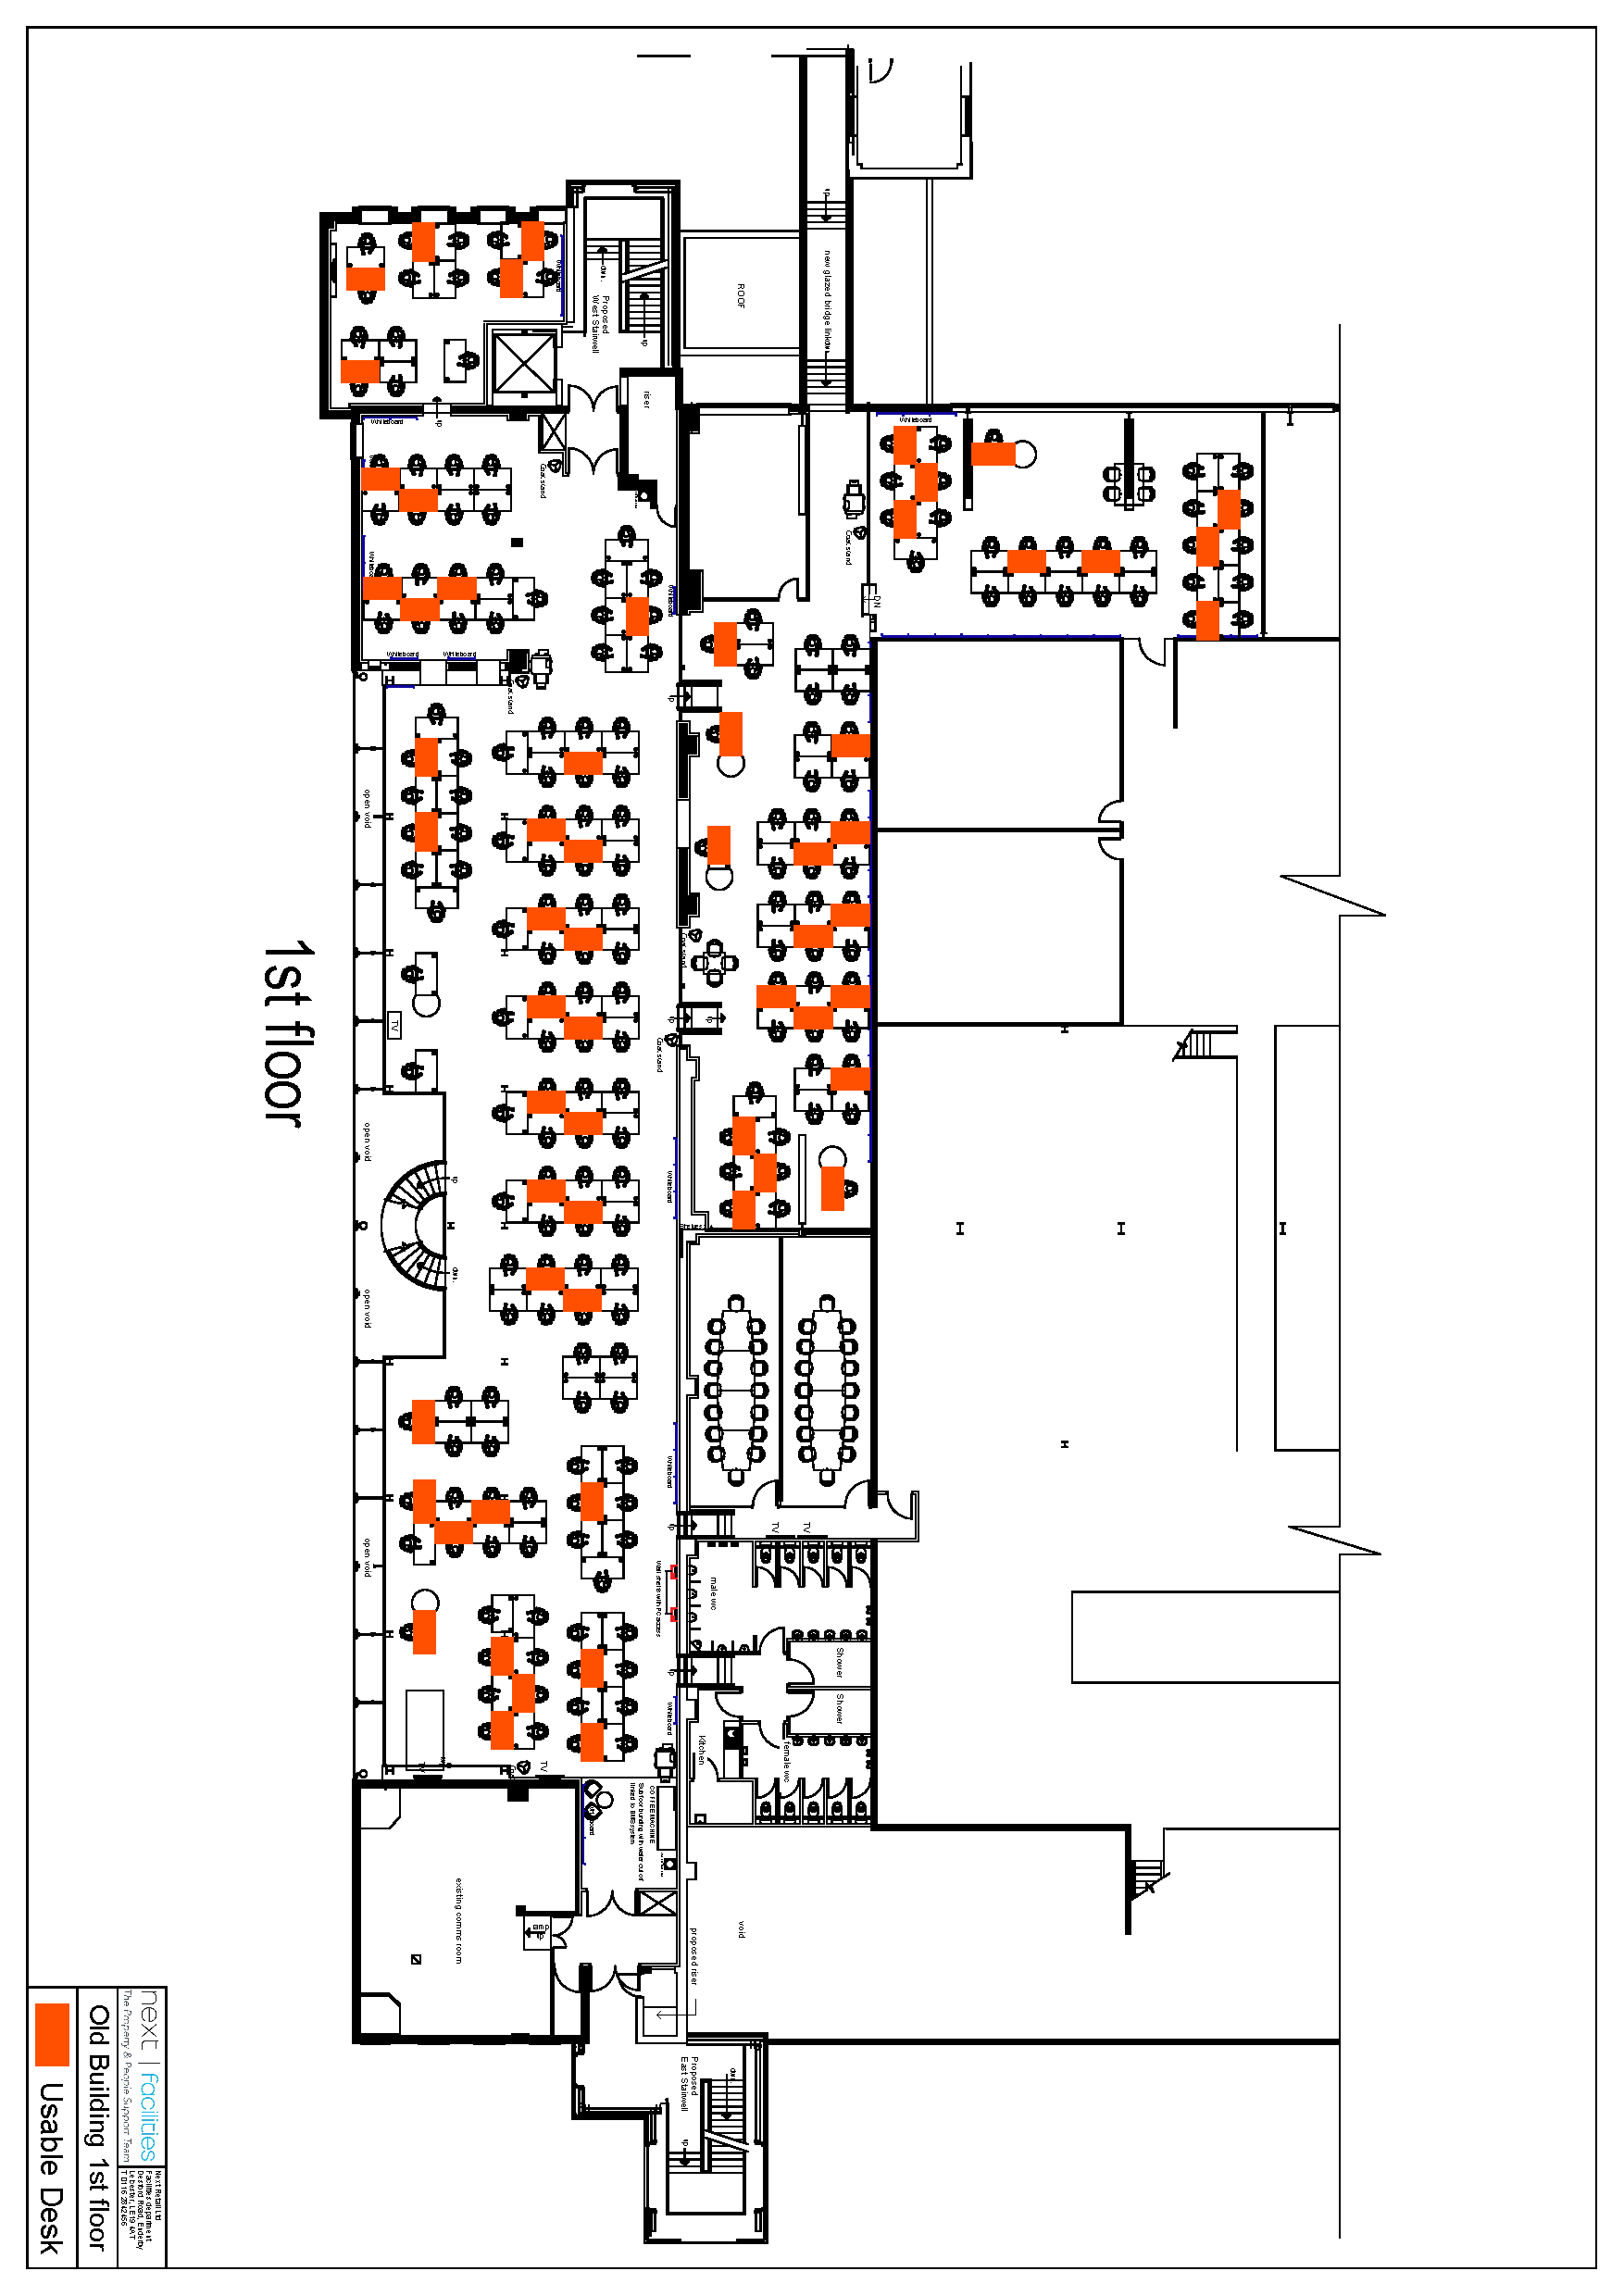
\includegraphics[scale = 0.36, angle = 90]{Old_building_1st_floor_usable_desks.pdf}
\caption{The seating arrangement given as an example in the CAD file, for reference.}
\label{Reference}
\end{subfigure}
~
\begin{subfigure}[h]{0.49\linewidth}
\centering
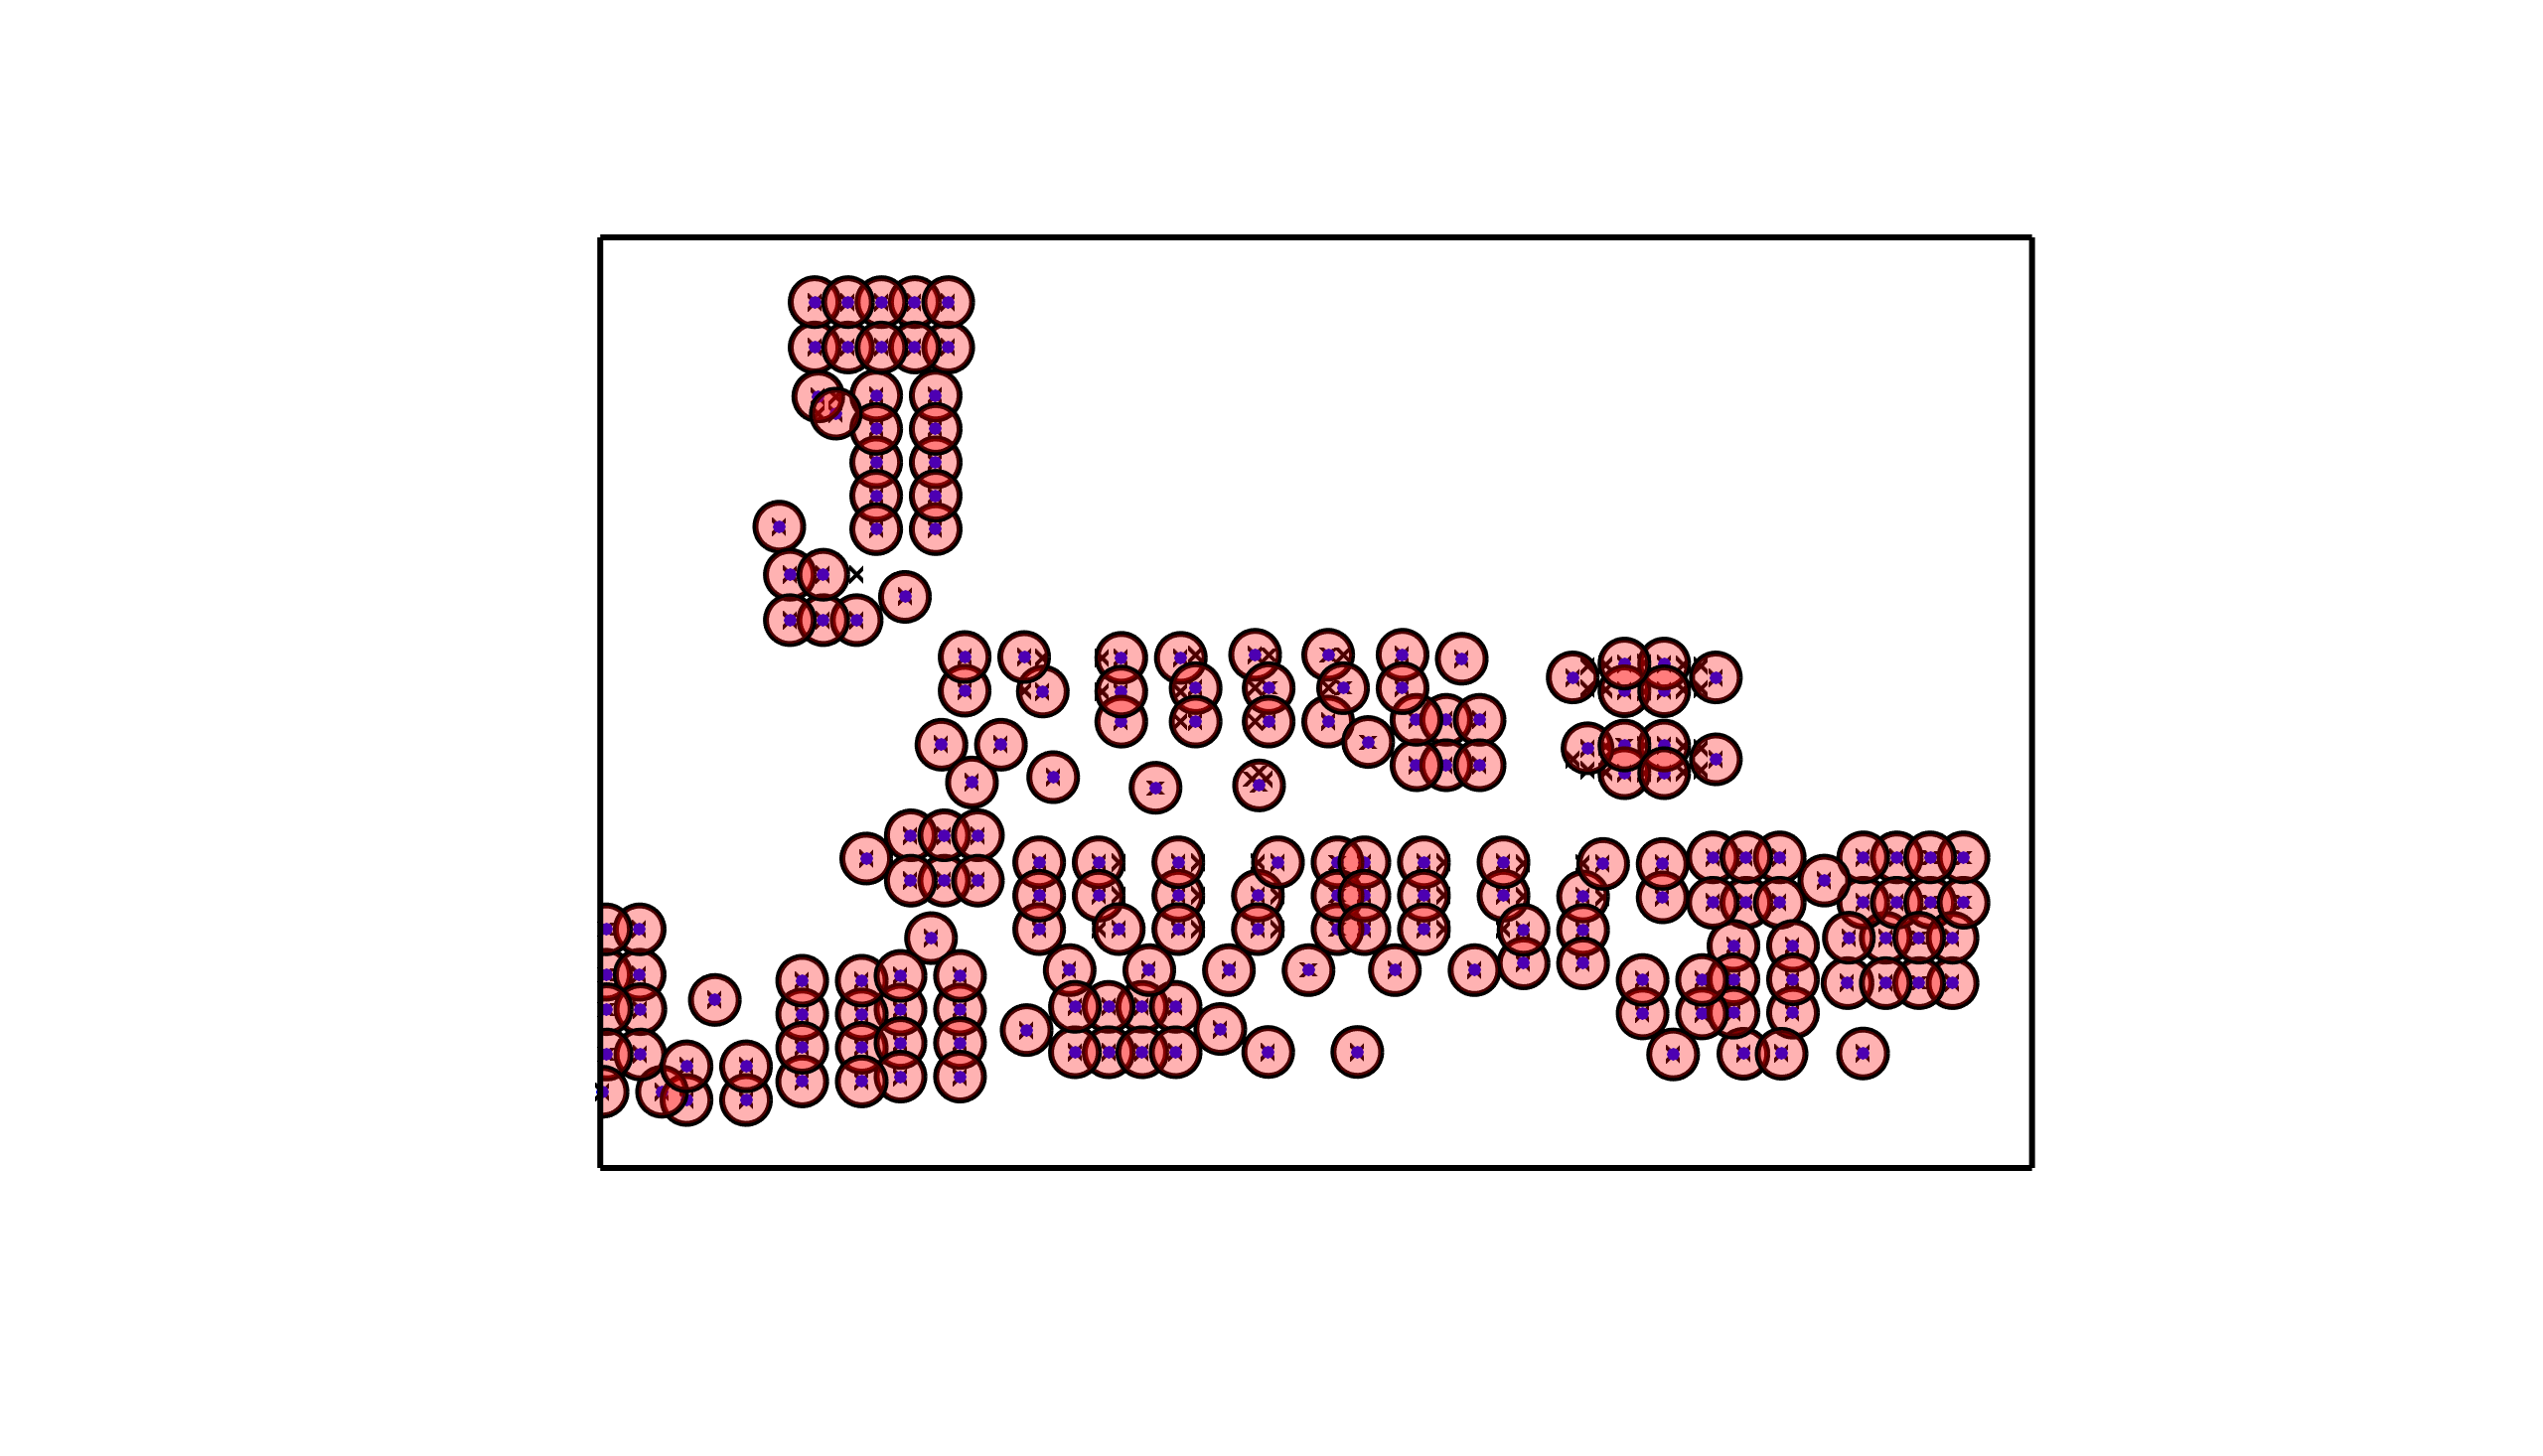
\includegraphics[width = \linewidth]{best_1m_next.png}
\caption{A sample layout for a social distancing measure of $1$ metres, which uses $201$ seats.}
\label{OneMetre}
\end{subfigure}
~
\begin{subfigure}[h]{0.490\linewidth}
\centering
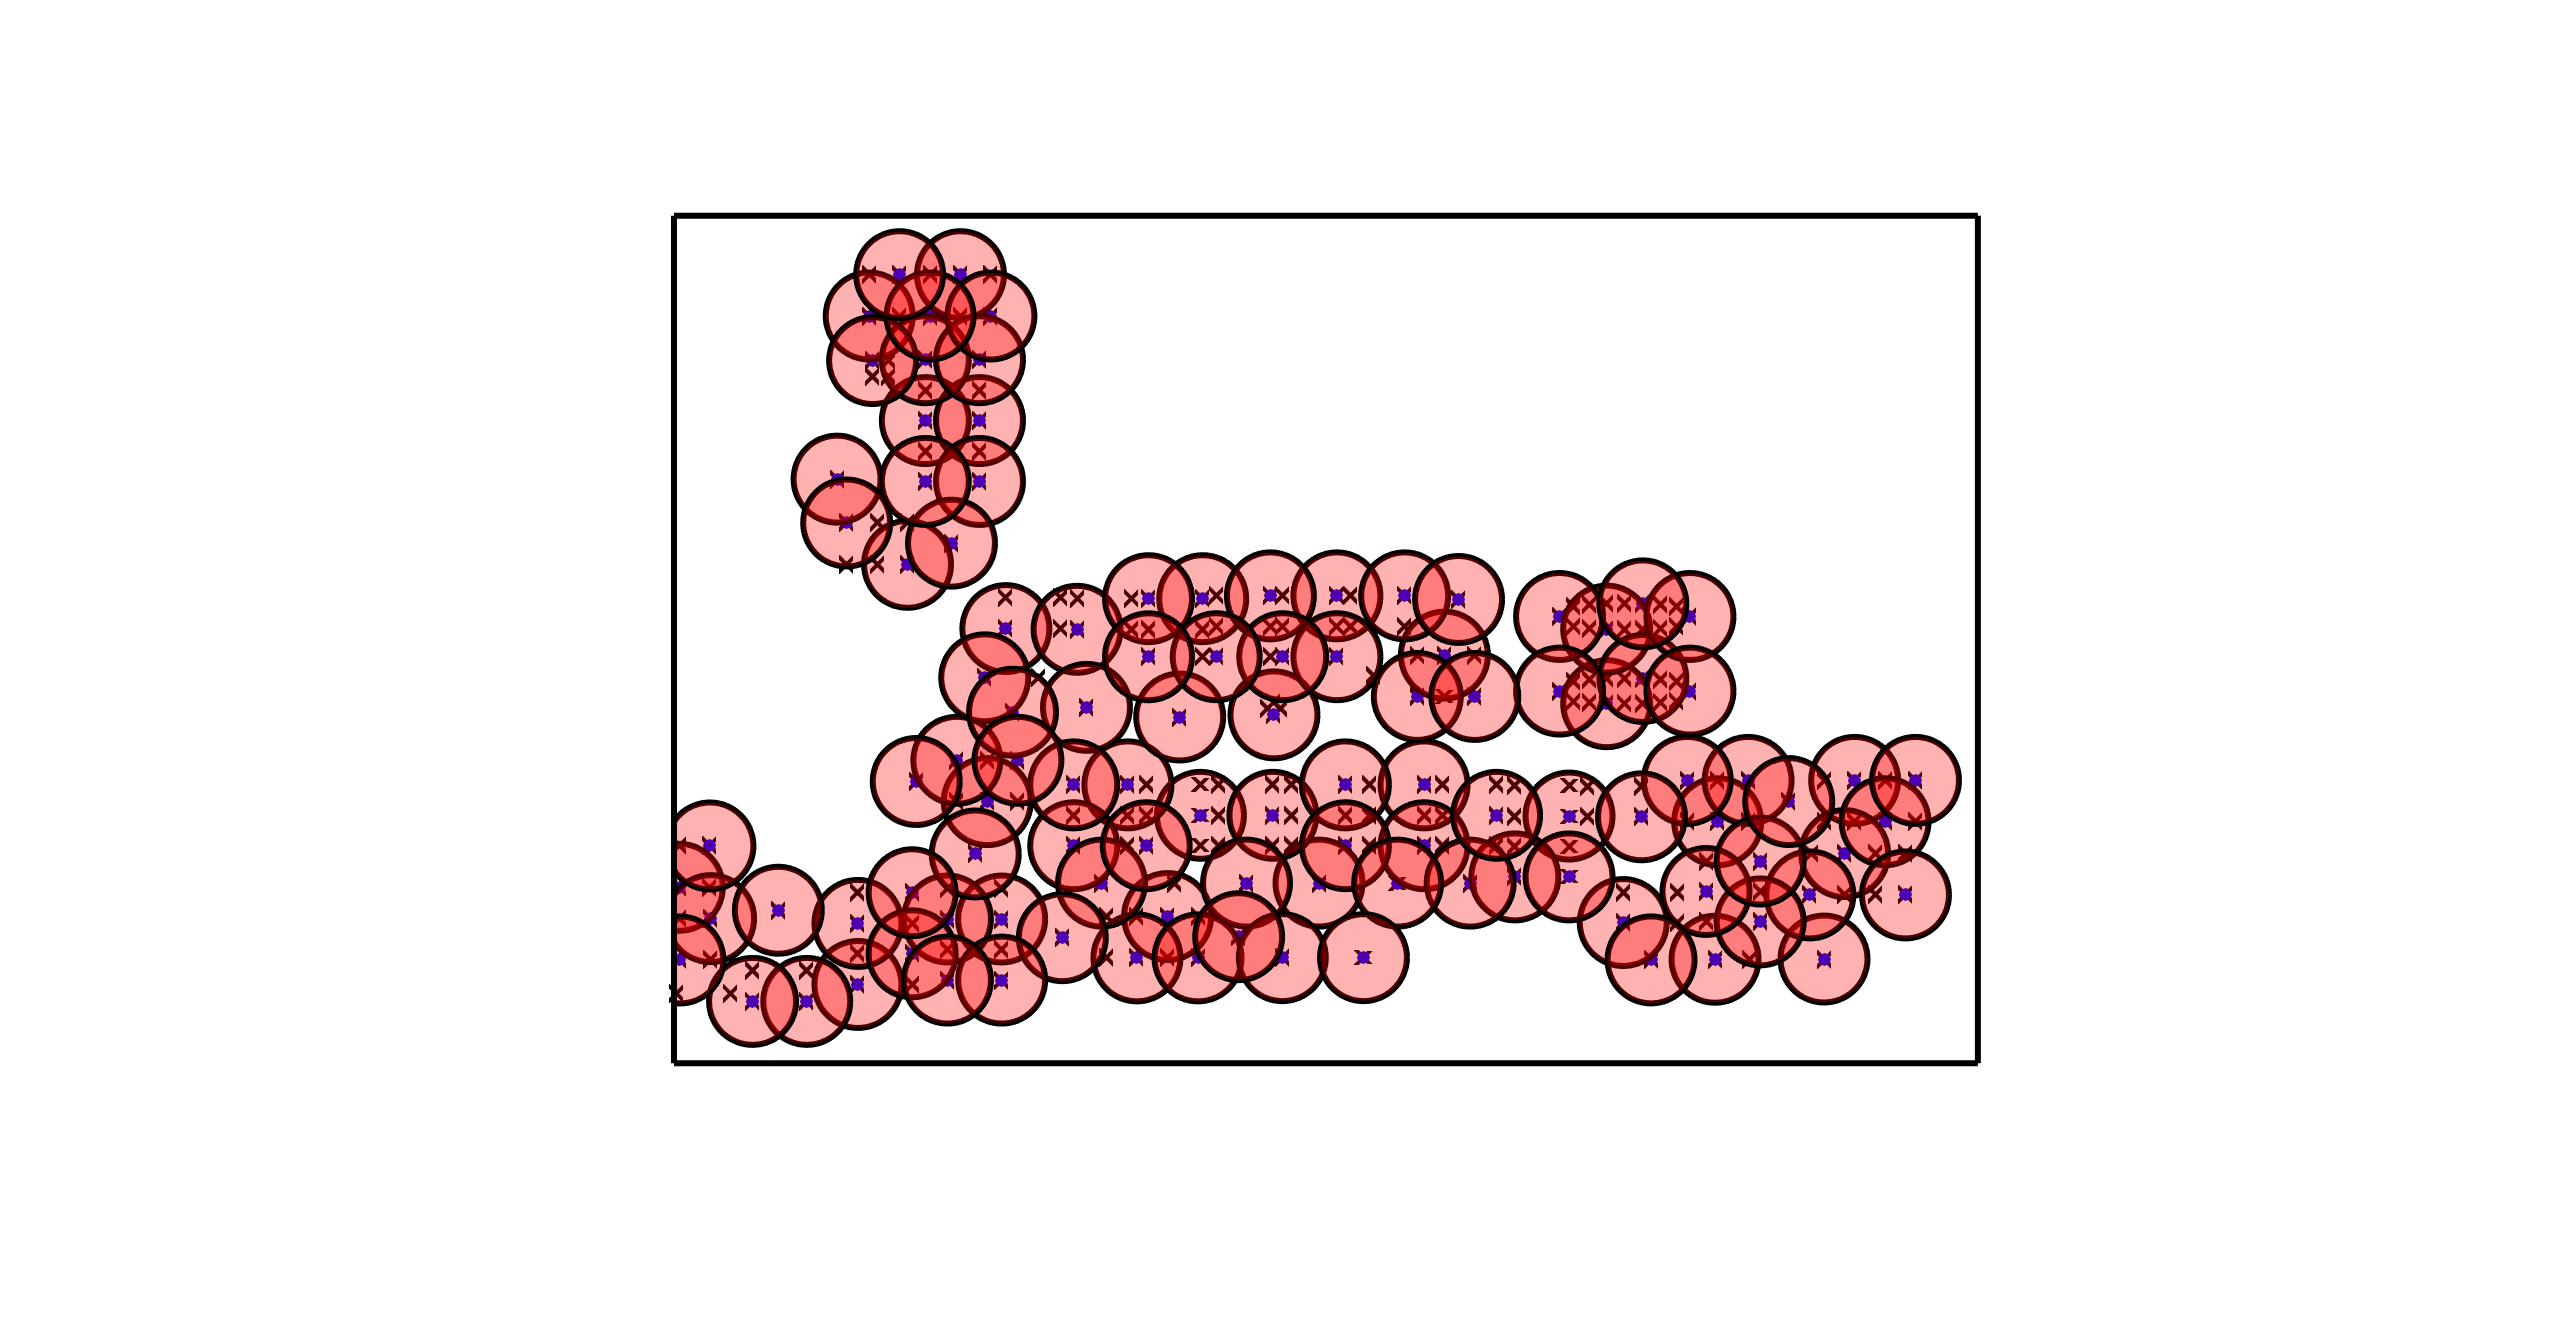
\includegraphics[width = \linewidth]{best_2m_next.png}
\caption{A sample layout for a social distancing measure of $2$ metres, which uses $105$ seats.}
\label{TwoMetre}
\end{subfigure}
\caption{A proposed office layout given by the app for $1$ and $2$ metre social distancing. Seat locations are marked with crosses, available seats are marked with dots and the `region of safety' is denoted by a circle around the available seats. Overlapping circles imply that certain regions are exposed to contamination from multiple sources, but no available seats are located in these regions. }
\label{Demonstration_pics}
\end{figure*}


\begin{table}[ht!]
\begin{center}
 \begin{tabular}{|c |c|} 
 \hline
& \textbf{Maximum capacity at $2$m social distancing (\%)}\\ 
 \hline
 Next CAD file benchmark &   27.9\\ 
 \hline
 Cardiff App  with conference rooms& 43.0\\
\hline
Cardiff App without conference rooms & 45.2\\
 \hline
\end{tabular}
\end{center}
\caption{Comparison of the performance of the Cardiff seat finding app against the benchmark provided in the supplied CAD file.}
\label{tab:performance}
\end{table}


As demonstrated in Table \ref{tab:performance}, we can very quickly achieve significantly higher occupancy rates in the office without violating social distancing measures. Given more time, we can search for even better solutions, as well as develop methods for user specification of shield locations (see first app).

\section*{Prospective developments for improving optimality}
Our app always provides seating arrangements that obey social distancing measures, and provides locally optimal solutions which are already better than the given benchmarks. Returning the  absolute optimum arrangement, however, is a lot more difficult because the problem is what is known as `NP-hard'.  Simply put, the only way to guarantee you have the most possible seats used is to try every possible order of seat checking, and pick the one which has the most seats used. Actually trying out every seat ordering would take a very long time; there are more ways to order $253$ seats than there are particles in the universe.\\

What we can do, though, is develop techniques to check our solutions and continuously improve upon them where possible. At a cost of additional time and computing power to implement, these methods would improve the likelihood we have found the best possible seating arrangement, allowing us to potentially further improve on our already powerful result. For example, we have a provided preliminary calculations in \autoref{fig:Stochastic_sims} to show that our current results are optimal up to 10,000 simulations, however, this can extended with computational power and theoretical applications.\\

\end{document}